\section{Atividade 6}
\subsection{Introdução ao Modelo com Controlador PID}
Os controladores PID são amplamente reconhecidos por sua eficácia e flexibilidade, combinando três elementos distintos para obter um desempenho superior: proporcional, integral e derivativo. Ao contrário dos controladores proporcionais, que ajustam a resposta do sistema de maneira direta ao erro atual, os controladores PID aproveitam três abordagens diferentes, cada uma desempenhando uma função específica.

O componente proporcional funciona de modo semelhante ao controlador proporcional simples, ajustando a saída do sistema em relação direta ao erro, com o objetivo de reduzir a diferença entre o valor medido e o valor desejado. No entanto, quando o componente proporcional sozinho não consegue corrigir totalmente o erro acumulado, entra em ação o componente integral, que soma e integra o erro ao longo do tempo para eliminá-lo.

Além disso, o componente derivativo desempenha um papel crucial ao prever mudanças no erro, ajudando a evitar que essas variações causem impactos negativos na saída do sistema. Com a integração desses três elementos, os controladores PID conseguem oferecer um controle mais preciso e estável, ajustando continuamente a saída para manter o sistema no estado desejado.
A fórmula padrão de um controlador PID pode ser representada pela equação \ref{eq:pid}:
\begin{equation}
    u(t) = K_p e(t) + K_i \int_{0}^{t} e(T) dT + K_d \frac{d e(t)}{dt}
    \label{eq:pid}
\end{equation}

O método de Ziegler-Nichols, desenvolvido por John G. Ziegler e Nathaniel B. Nichols, é uma técnica consolidada para a sintonia de controladores PID. Este método é particularmente útil porque simplifica a configuração dos controladores ao fornecer fórmulas práticas para calcular os ganhos \( K_p \), \( K_i \), e \( K_d \) com base na resposta do sistema a uma entrada de teste. Esses parâmetros são ajustados para otimizar a resposta do sistema em termos de tempo de subida, sobreposição e tempo de assentamento.

Os valores dos ganhos são estabelecidos de acordo com a estabilidade observada do sistema e são tipicamente calculados a partir do ganho crítico \( K_c \) e do período crítico \( P_c \), que são obtidos através de testes de malha aberta. A Tabela \ref{tab:ziegler-nichols} resume os valores recomendados para cada tipo de ganho:

\begin{table}[h]
    \centering
    \begin{tabular}{ccc}
        \hline
        \( K_p \)            & \( K_i \)                      & \( K_d \)              \\
        \hline
        \( 0,6 \times K_c \) & \( \frac{2 \times K_p}{P_c} \) & \( 0,125 \times P_c \) \\
        \hline
    \end{tabular}
    \caption{Valores dos ganhos segundo o método de Ziegler-Nichols}
    \label{tab:ziegler-nichols}
\end{table}

Baseando-se nas análises realizadas na Atividade 4, foi possível determinar um valor limite para o ganho crítico \( K_c \) de 14.93. Esta descoberta é essencial para o ajuste dos parâmetros do controlador PID segundo o método de Ziegler-Nichols.

\begin{figure}[H]
    \centering
    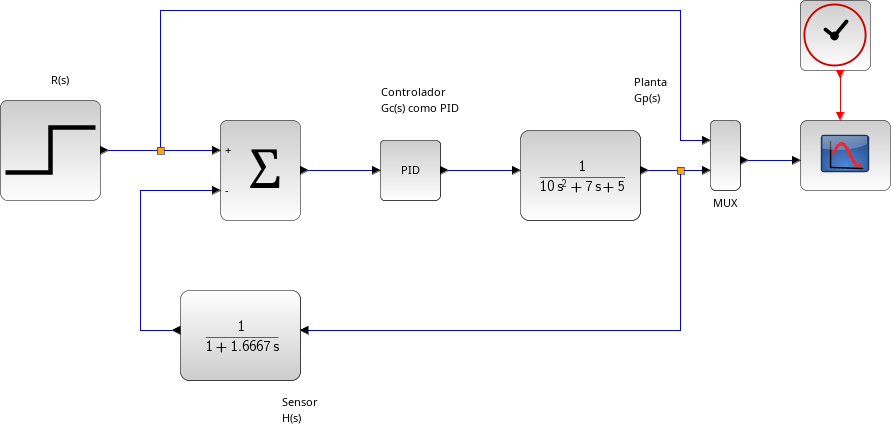
\includegraphics[width=0.7\textwidth]{6-atividade/assets/diagrama-a.png}
    \caption{Diagrama mostrando o sistema no ponto crítico com \( K_c = 14.93 \)}
    \label{fig:diagrama-ponto-critico}
\end{figure}

A simulação realizada com \( K_c = 14.93 \) demonstrou que o sistema alcança um estado crítico, como evidenciado no gráfico abaixo:


\begin{figure}[H]
    \centering
    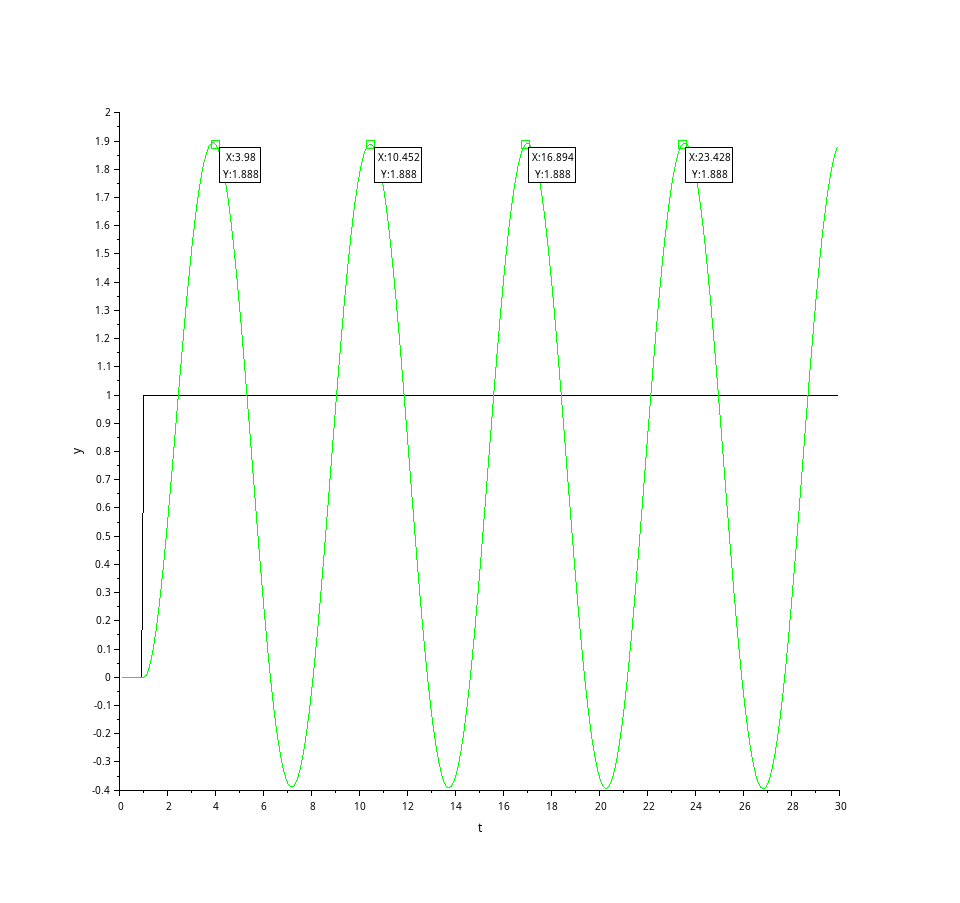
\includegraphics[width=0.7\textwidth]{6-atividade/assets/instavel-posicao-sistema-controlador.png}
    \caption{Resposta do sistema com o controlador PID ajustado para \( K_c = 14.93 \)}
    \label{fig:resposta-sistema-controlador}
\end{figure}


A resposta simulada revela claramente o comportamento do sistema na condição de ganho crítico, possibilitando a utilização desses dados para calibrar os parâmetros do controlador PID, garantindo eficiência e estabilidade no controle do sistema.


\subsection{Determinação dos Parâmetros do Controlador PID}
Após identificarmos o ganho crítico \( K_c = 14.93 \) através de análises detalhadas, o que nos permite empregar o método de Ziegler-Nichols para ajustar os parâmetros do controlador PID. Este método é eficaz para sintonizar controladores em sistemas onde a resposta precisa ser otimizada em termos de estabilidade e rapidez.

\subsection{Cálculo dos Parâmetros do Controlador PID}
O método de Ziegler-Nichols é conhecido por sua eficiência na configuração inicial de controladores PID. Ele utiliza o ganho crítico \( K_c \) e o período crítico \( P_c \) para estabelecer os parâmetros de controle, ajustando assim a resposta do sistema.

\begin{itemize}
    \item \textbf{Ganho Proporcional} \( K_p \):
          \[
              K_p = 0.6 \times K_c = 0.6 \times 14.93 \approx 8.958
          \]
    \item \textbf{Ganho Integral} \( K_i \) (assumindo um \( P_c \) conhecido de 10 segundos para exemplificação):
          \[
              K_i = \frac{2 \times K_p}{P_c} = \frac{2 \times 8.958}{10} \approx 1.7916
          \]
    \item \textbf{Ganho Derivativo} \( K_d \):
          \[
              K_d = 0.125 \times P_c = 0.125 \times 10 = 1.25
          \]
\end{itemize}

\subsection{Implementação e Validação dos Parâmetros}
Os parâmetros \( K_p = 8.958 \), \( K_i = 1.7916 \), e \( K_d = 1.25 \) são implementados no controlador PID no ambiente de simulação, como Scilab. Esses valores são projetados para ajustar o sistema para responder de forma ideal em várias condições operacionais, melhorando a estabilidade e precisão do sistema.

A eficácia desses parâmetros será validada por meio de simulações subsequentes, as quais confirmarão se eles mantêm o desempenho desejado do sistema, garantindo que o controle PID seja tanto eficiente quanto efetivo.

\begin{figure}[H]
    \centering
    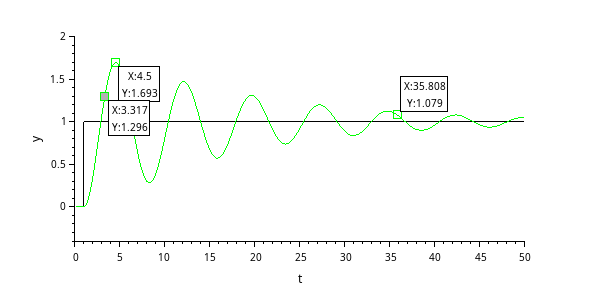
\includegraphics[width=0.8\textwidth]{6-atividade/assets/pid-valores-iniciais.png}
    \caption{Resposta do sistema com os parâmetros do PID ajustados.}
    \label{fig:resposta-pid}
\end{figure}

Após a validação inicial, um refinamento manual dos parâmetros pode ser necessário para otimizar ainda mais a resposta do sistema. Este processo de ajuste fino baseia-se na análise das respostas obtidas e na experiência prática, permitindo uma sintonia mais precisa que responde de maneira adequada às especificidades do sistema e às variações nas condições operacionais. Este ajuste fino é crucial para alcançar a melhor performance, equilibrando a estabilidade e a rapidez da resposta do controlador PID.

Subsequentemente, novas simulações serão realizadas para validar a eficácia dos parâmetros ajustados. Essa etapa é crucial para verificar se os ajustes refinados mantêm a saída do sistema próxima ao valor desejado sob uma gama mais ampla de condições operacionais, garantindo a eficácia e a eficiência do controlador.

\subsection{Refinamento dos Parâmetros do Controlador PID}
Os parâmetros iniciais \( K_p \), \( K_i \), e \( K_d \) obtidos pelo método de Ziegler-Nichols, baseados no ganho crítico estimado de \( K_c = 14.93 \), fornecem um ponto de partida útil para a configuração do controlador PID. No entanto, a precisão inicial na estimativa de \( K_c \) pode influenciar diretamente a eficácia destes parâmetros, necessitando de ajustes refinados para alinhar o desempenho do controlador às características específicas do sistema.

\begin{itemize}
    \item \textbf{Ajuste do Ganho Proporcional (\( K_p \))}: O valor inicial de \( K_p = 8.9754 \) pode precisar ser ajustado se a resposta do sistema for muito lenta ou rápida demais, o que indica que a estimativa de \( K_c \) pode não ter capturado perfeitamente as dinâmicas do sistema.
    \item \textbf{Ajuste do Ganho Integral (\( K_i \))}: Da mesma forma, o valor de \( K_i = 1.79508 \) (calculado com um \( P_c \) hipotético de 10) pode requerer modificações para otimizar a correção de erros de longo prazo, sugerindo que a sensibilidade do sistema a erros acumulados pode ter sido subestimada.
    \item \textbf{Ajuste do Ganho Derivativo (\( K_d \))}: O valor inicial de \( K_d = 1.25 \) pode também necessitar de ajustes para melhor controlar a resposta do sistema a mudanças rápidas nas condições de entrada ou perturbações.
\end{itemize}

\subsection{Testes de Refinamento do Controlador PID}
Para otimizar ainda mais o desempenho do controlador PID e garantir a eficiência e eficácia do sistema sob várias condições operacionais, procederemos com uma série de testes. Nestes testes, focaremos inicialmente em ajustar o ganho proporcional \( K_p \) enquanto mantemos os valores de \( K_i \) e \( K_d \) fixos, a fim de entender o impacto de \( K_p \) na resposta dinâmica do sistema.

\subsubsection{Configuração dos Testes}
Os testes são configurados para variar \( K_p \) em uma faixa específica enquanto \( K_i \) e \( K_d \) são mantidos constantes nos valores calculados anteriormente. Essa abordagem permite observar como ajustes no ganho proporcional afetam características como o tempo de subida, o sobressinal e o tempo de assentamento do sistema.

\subsubsection{Resultados dos Testes}
Os resultados desses testes são apresentados através de gráficos que mostram a resposta do sistema a uma entrada de degrau padrão para diferentes valores de \( K_p \). Cada gráfico ilustrará como as variações em \( K_p \) influenciam o desempenho do sistema, destacando a eficácia do ajuste do ganho proporcional em melhorar a resposta do controlador.


Esse aqui é o diagrama
\begin{figure}[H]
    \centering
    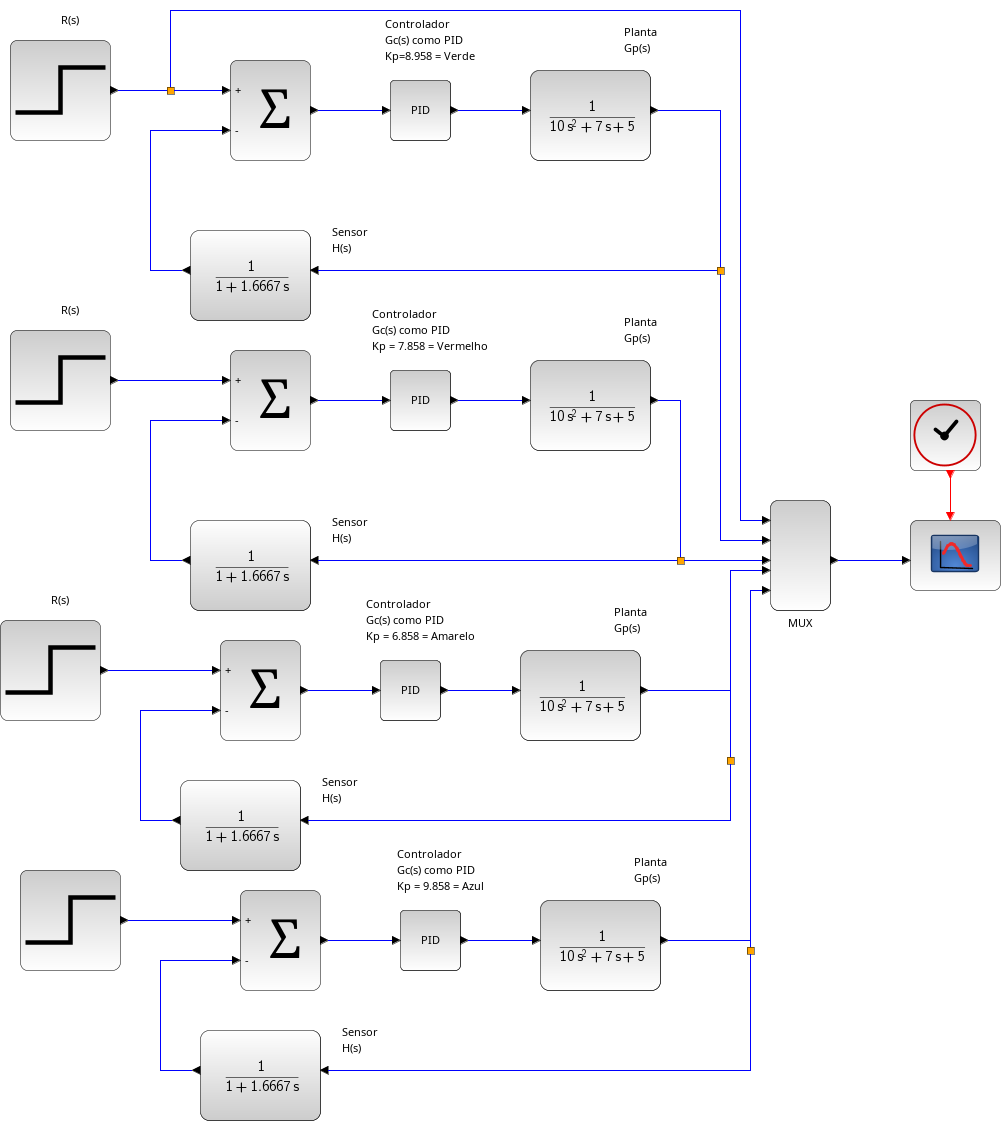
\includegraphics[width=0.8\textwidth]{6-atividade/assets/diagrama-pid-ajustando-kp.png}
    \caption{Resposta do sistema para diferentes valores de \( K_p \) com \( K_i \) e \( K_d \) fixos.}
    \label{fig:diagrama-pid-ajustando-kp}
\end{figure}

agora o resultado
\begin{figure}[H]
    \centering
    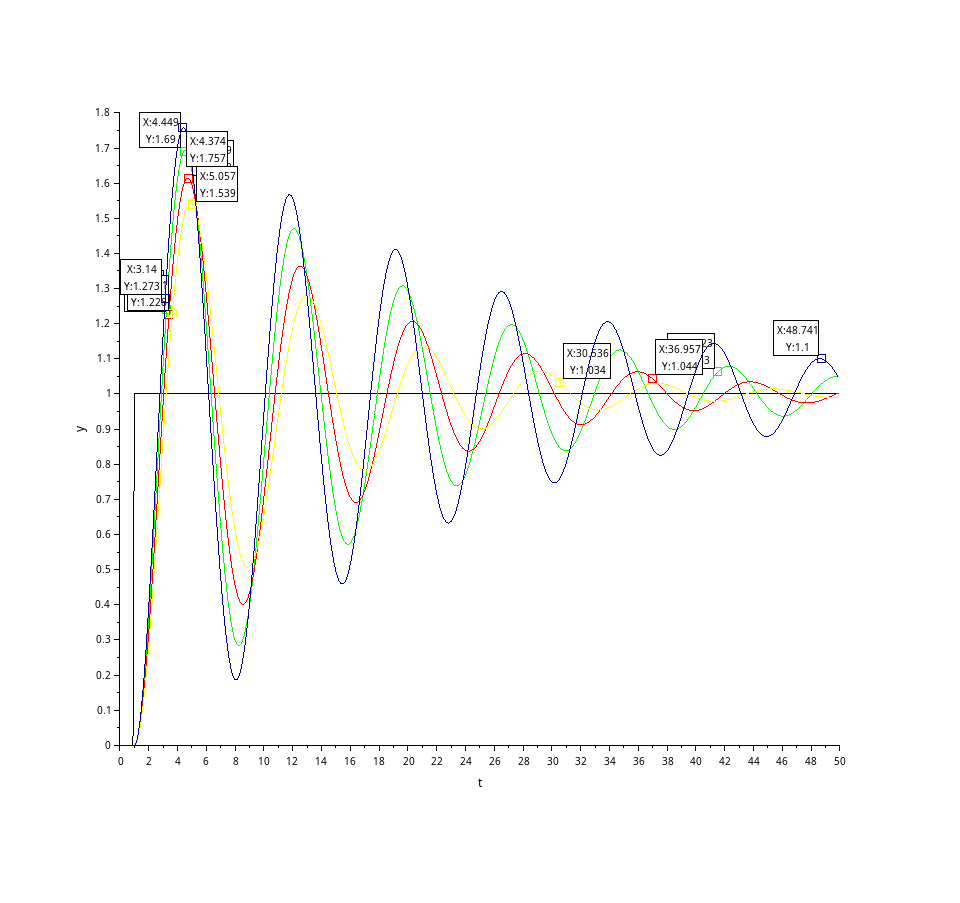
\includegraphics[width=0.8\textwidth]{6-atividade/assets/pid-ajustando-kp.png}
    \caption{Resposta do sistema para diferentes valores de \( K_p \) com \( K_i \) e \( K_d \) fixos.}
    \label{fig:pid-ajustando-kp}
\end{figure}

\subsubsection{Resultados dos Testes de Variação de \( K_p \)}
O gráfico a seguir apresenta a resposta do sistema para quatro diferentes configurações de \( K_p \), com \( K_i \) e \( K_d \) mantidos constantes. Cada curva representa uma tentativa distinta de ajustar a rapidez e o amortecimento da resposta do sistema através da modificação do ganho proporcional.

\subsubsection{Discussão dos Resultados}
A análise visual das respostas mostra que:
\begin{itemize}
    \item A curva azul (\( K_p = 9.858 \)) apresenta maior sobressinal e oscilações prolongadas, indicando uma resposta potencialmente muito agressiva.
    \item A curva amarela (\( K_p = 6.858 \)) e a vermelha (\( K_p = 7.858 \)) mostram menor sobressinal, mas ainda com oscilações visíveis, sugerindo uma melhoria em estabilidade em comparação ao azul.
    \item A curva verde (\( K_p = 8.858 \)), que é a configuração padrão, oferece um equilíbrio entre rápida estabilização e controle de oscilações, possivelmente representando a configuração mais eficaz entre as testadas.
\end{itemize}

\subsubsection{Conclusões dos Testes}
Estes resultados indicam que ajustes finos em \( K_p \) podem significativamente alterar a dinâmica do sistema. O valor de \( K_p = 8.858 \) parece oferecer o melhor compromisso entre estabilidade e tempo de resposta, fazendo dele uma escolha preferencial para futuras configurações do controlador PID neste sistema específico.


\subsubsection{Testes de Variação de \( K_i \)}
Nesta série de testes, exploramos o impacto de ajustes no ganho integral \( K_i \) enquanto mantemos \( K_p \) e \( K_d \) fixos. O objetivo é observar como variações em \( K_i \) influenciam a capacidade do sistema de eliminar o erro estático e estabilizar a resposta ao longo do tempo.
\subsection{Refinamento dos Parâmetros do Controlador PID}
Os parâmetros iniciais \( K_p \), \( K_i \), e \( K_d \) obtidos pelo método de Ziegler-Nichols, baseados no ganho crítico estimado de \( K_c = 14.959 \), fornecem um ponto de partida útil para a configuração do controlador PID. No entanto, para refinar esses parâmetros, realizamos uma série de testes variando o ganho integral \( K_i \) enquanto mantemos \( K_p \) e \( K_d \) fixos. O objetivo é avaliar como ajustes em \( K_i \) afetam a estabilidade e a rapidez da resposta do sistema.

\begin{figure}[H]
    \centering
    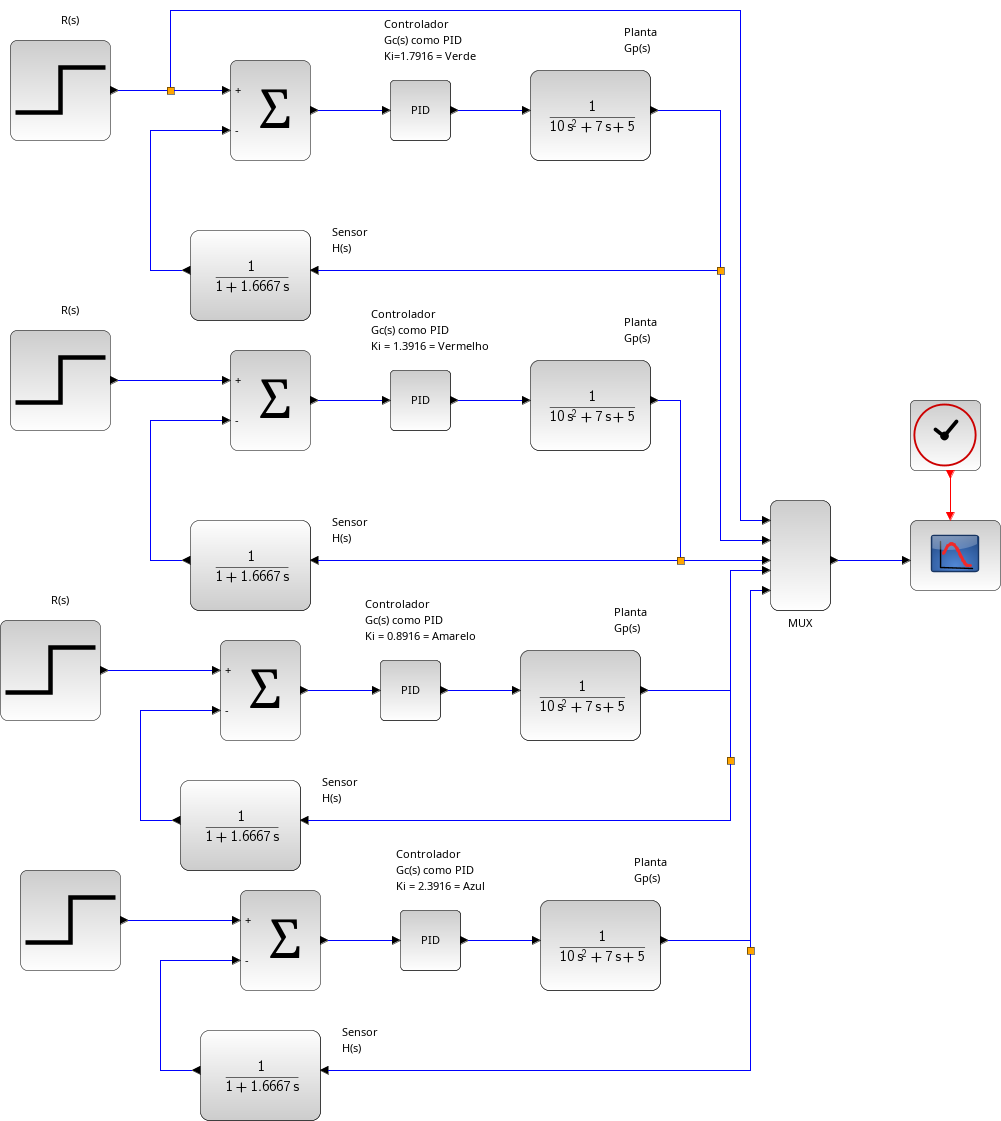
\includegraphics[width=0.8\textwidth]{6-atividade/assets/diagrama-pid-ajustando-ki.png}
    \caption{Diagrama do sistema com diferentes configurações de \( K_i \).}
    \label{fig:diagram-pid-adjusting-ki}
\end{figure}

\begin{figure}[H]
    \centering
    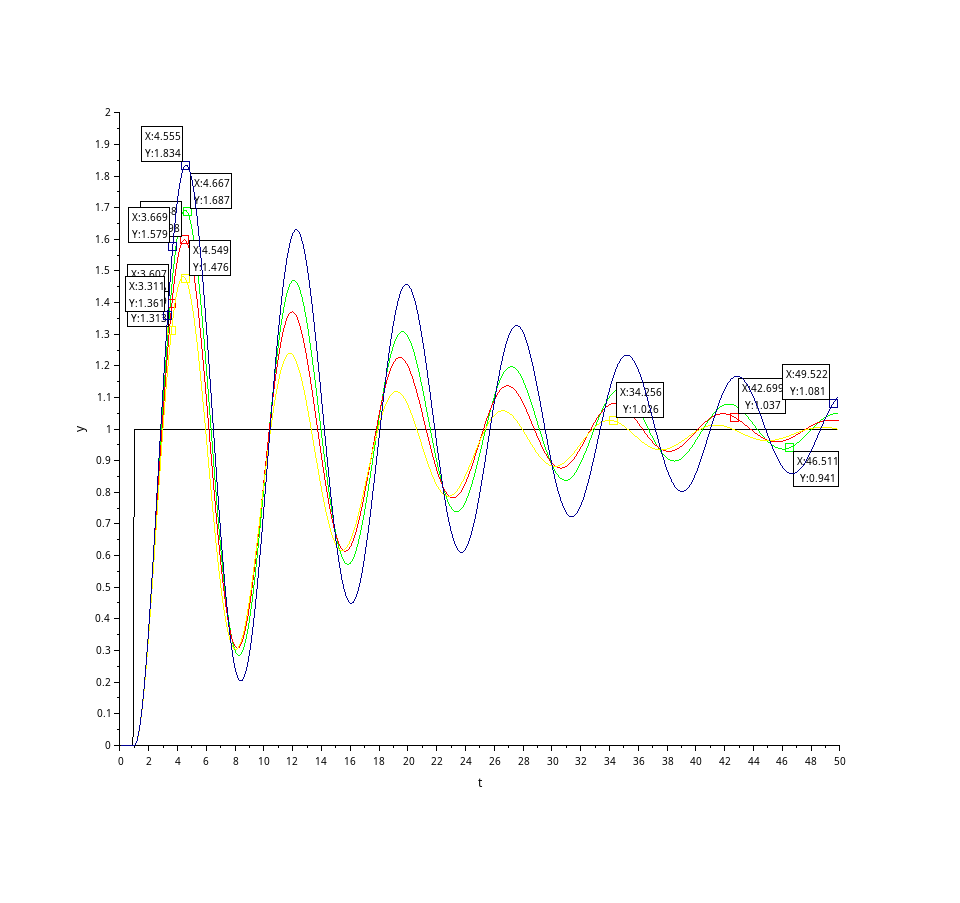
\includegraphics[width=0.8\textwidth]{6-atividade/assets/pid-ajustando-ki.png}
    \caption{Resposta do sistema para diferentes valores de \( K_i \) com \( K_p \) e \( K_d \) fixos. As cores representam diferentes valores de \( K_i \): verde para \( K_i = 1.7916 \), vermelho para \( K_i = 1.3916 \), amarelo para \( K_i = 0.8916 \), e azul para \( K_i = 2.3916 \).}
    \label{fig:response-various-ki}
\end{figure}

\subsubsection{Discussão dos Resultados}
A análise dos gráficos revela:
\begin{itemize}
    \item A curva verde (\( K_i = 1.7916 \)) apresenta uma resposta rápida e estabilizada, indicando um ajuste eficaz para as condições atuais do sistema.
    \item As curvas vermelha (\( K_i = 1.3916 \)) e amarela (\( K_i = 0.8916 \)) exibem respostas mais lentas e menos eficientes para eliminar o erro permanente.
    \item A curva azul (\( K_i = 2.3916 \)) tende a oscilar excessivamente, sugerindo que um valor de \( K_i \) mais elevado pode induzir instabilidade.
\end{itemize}

\subsubsection{Conclusões dos Testes}
Os testes indicam que um ajuste cuidadoso de \( K_i \) é crucial para otimizar a resposta do sistema. O valor de \( K_i = 1.7916 \) se mostrou mais adequado, equilibrando a redução do erro permanente com uma resposta estável. Estes resultados serão usados para recomendar ajustes finais nos parâmetros do controlador PID, assegurando que ele opere eficientemente sob as condições esperadas.

\subsection{Ajuste do Ganho Derivativo}
Com os ganhos proporcional \( K_p \) e integral \( K_i \) fixados, conduzimos uma série de testes alterando o ganho derivativo \( K_d \) para observar seu impacto na dinâmica de resposta do sistema. Estes testes ajudam a entender melhor como o ajuste fino de \( K_d \) pode controlar as oscilações e melhorar a estabilidade do sistema.

\begin{figure}[H]
    \centering
    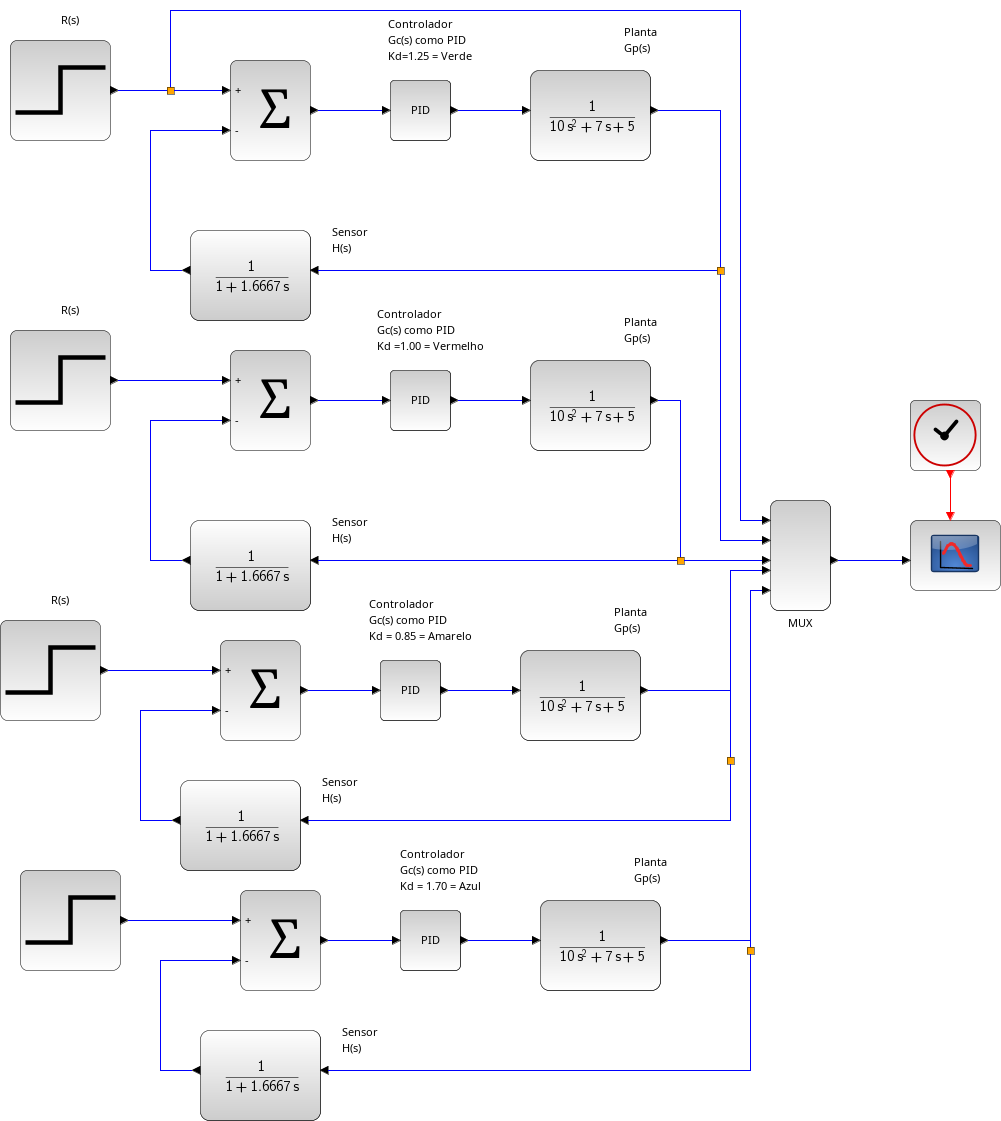
\includegraphics[width=0.8\textwidth]{6-atividade/assets/diagrama-pid-ajustando-kd.png}
    \caption{Diagrama do sistema com diferentes configurações de \( K_d \).}
    \label{fig:diagram-pid-adjusting-kd}
\end{figure}

\begin{figure}[H]
    \centering
    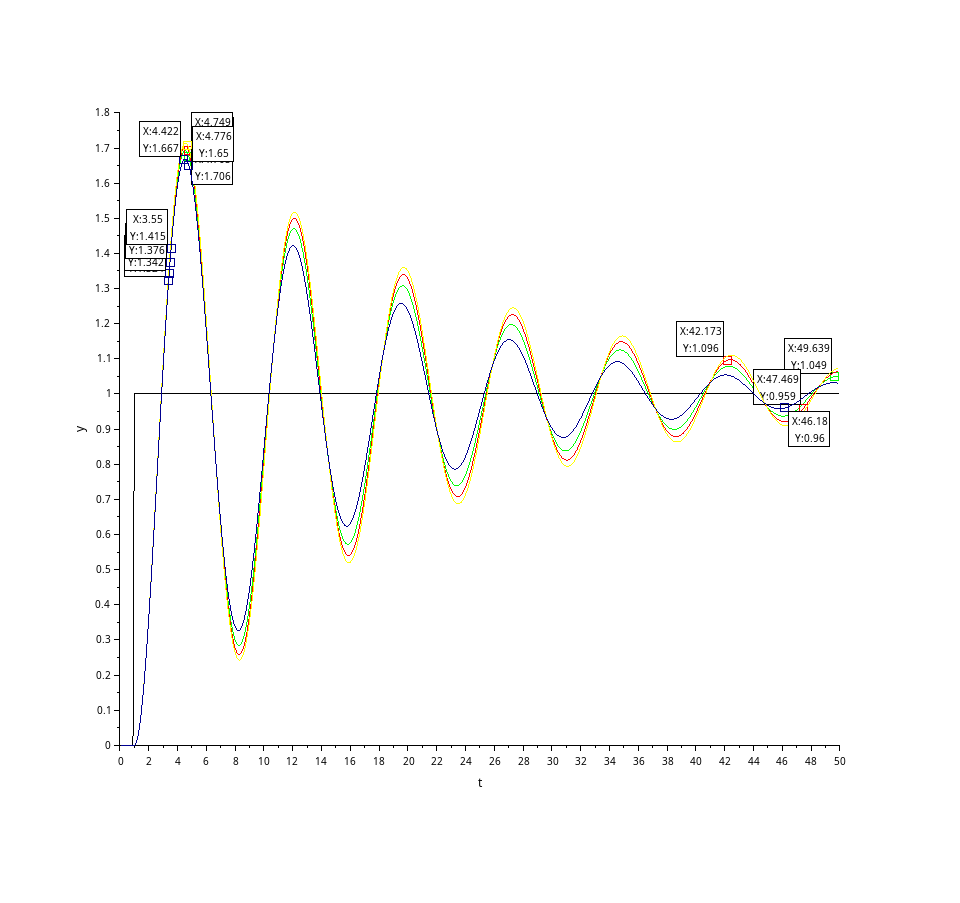
\includegraphics[width=0.8\textwidth]{6-atividade/assets/pid-ajustando-kd.png}
    \caption{Resposta do sistema para diferentes valores de \( K_d \) com \( K_p \) e \( K_i \) fixos. As cores representam diferentes valores de \( K_d \): verde para \( K_d = 1.25 \), vermelho para \( K_d = 1.00 \), amarelo para \( K_d = 0.85 \), e azul para \( K_d = 1.70 \).}
    \label{fig:response-various-kd}
\end{figure}

\subsubsection{Discussão dos Resultados}
A análise dos gráficos indica:
\begin{itemize}
    \item A curva verde (\( K_d = 1.25 \)) apresenta uma resposta equilibrada, com oscilações moderadas e rápido tempo de assentamento.
    \item As curvas vermelha (\( K_d = 1.00 \)) e amarela (\( K_d = 0.85 \)) mostram maior oscilação e um tempo de assentamento mais prolongado, indicando menor eficácia no controle de perturbações rápidas.
    \item A curva azul (\( K_d = 1.70 \)) tem o menor sobressinal, indicando que um valor mais alto de \( K_d \) pode suprimir oscilações eficientemente, mas pode também resultar em uma resposta mais lenta.
\end{itemize}

\subsubsection{Conclusões dos Testes}
Os resultados sugerem que um \( K_d \) entre 1.25 e 1.70 proporciona uma boa compensação entre estabilidade e rapidez na resposta. Valores mais baixos de \( K_d \) resultam em maior oscilação, enquanto valores mais altos podem atrasar a resposta do sistema. Estes insights são cruciais para o ajuste final do controlador PID, garantindo uma operação eficaz e eficiente do sistema.
